
\documentclass[14pt]{extreport}
\usepackage{gost}
\usepackage{hyperref}
\usepackage{makecell}
\usepackage{ragged2e}
\justifying

\makeatletter
\@addtoreset{figure}{part}
\makeatother
\renewcommand{\thefigure}{\arabic{figure}}
\renewcommand{\thetable}{\arabic{table}}




\begin{document}
\pagestyle{empty} 
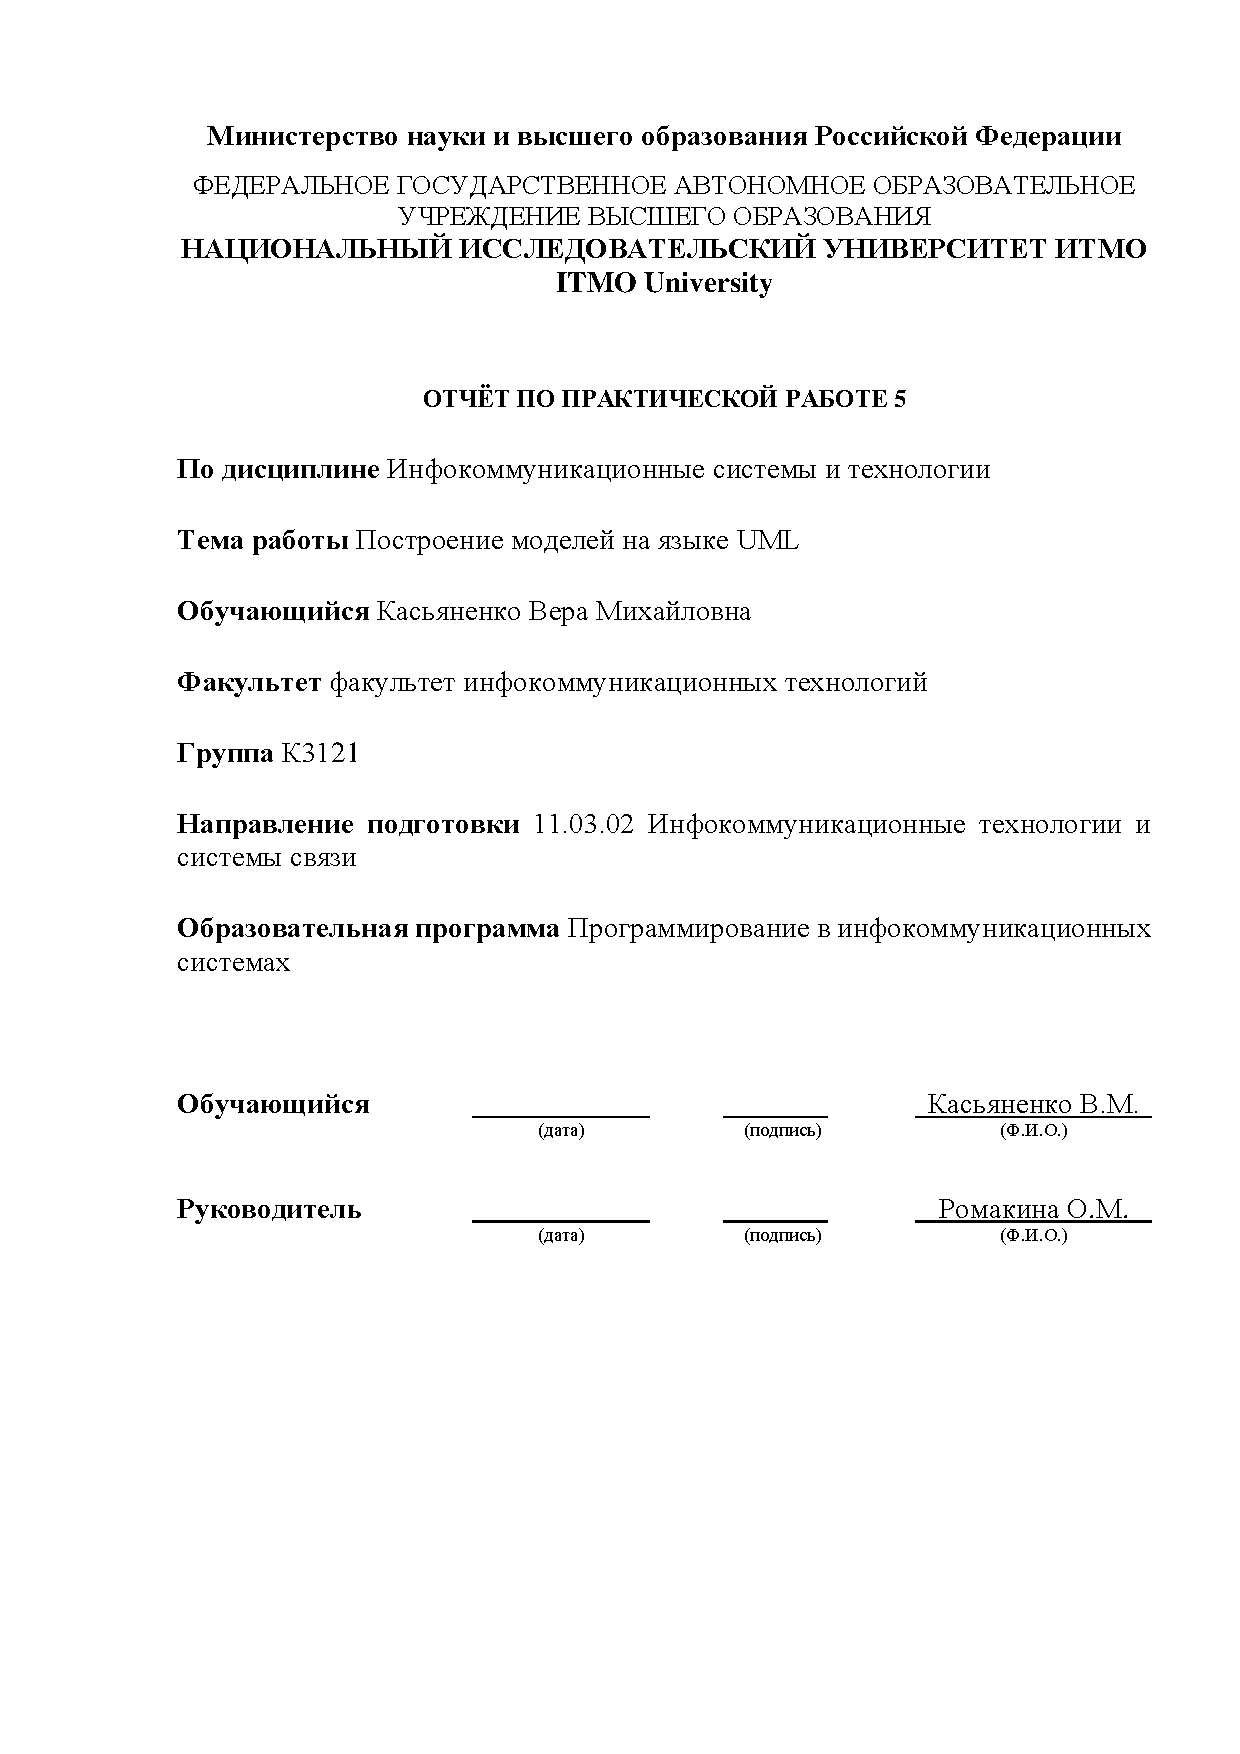
\includepdf[pages=-,pagecommand={}]{titulCourse.pdf}

\pagestyle{plain}
\tableofcontents
 



\intro 

В данном отчете будут представлены диаграммы активности и вариантов
использования мобильного приложения OptiTune на языке UML, а также будут рассмотрены альтернативные потоки событий для основных прецедентов.


\chapter{Диаграммы UML\label{chapter1}}
\section{Диаграммы прецедентов на языке UML}

В данном разделе представлены диаграммы прецедентов на языке UML. Для более удобного восприятия они были разделены на диаграммы для незарегистированных (рисунок \ref{fig1}) и зарегистрированных пользователей (рисунок \ref{fig2}), а также для членов административной группы (рисунок \ref{fig3}).

\begin{figure}[H]
\centerline{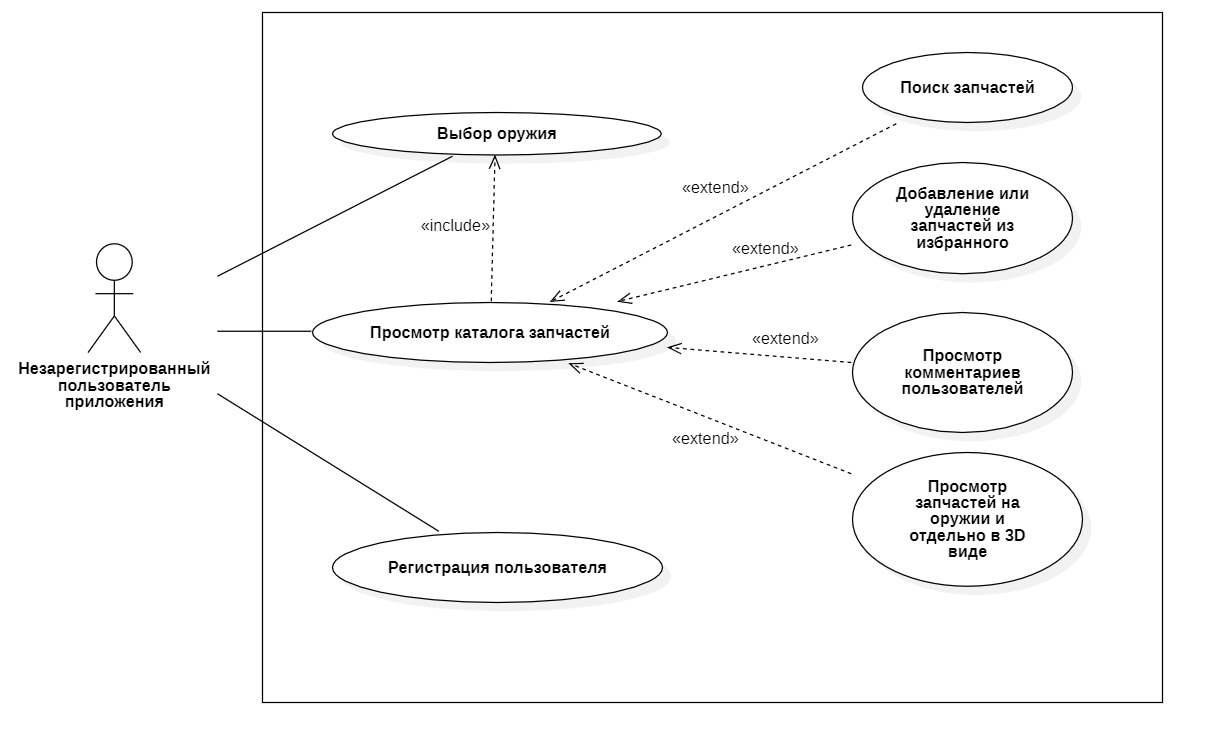
\includegraphics[width=1\linewidth]{nereg}}
\caption{Диаграмма прецедентов для пользователей без регистрации}
\label{fig1}
\end{figure}

\begin{figure}[H]
\centerline{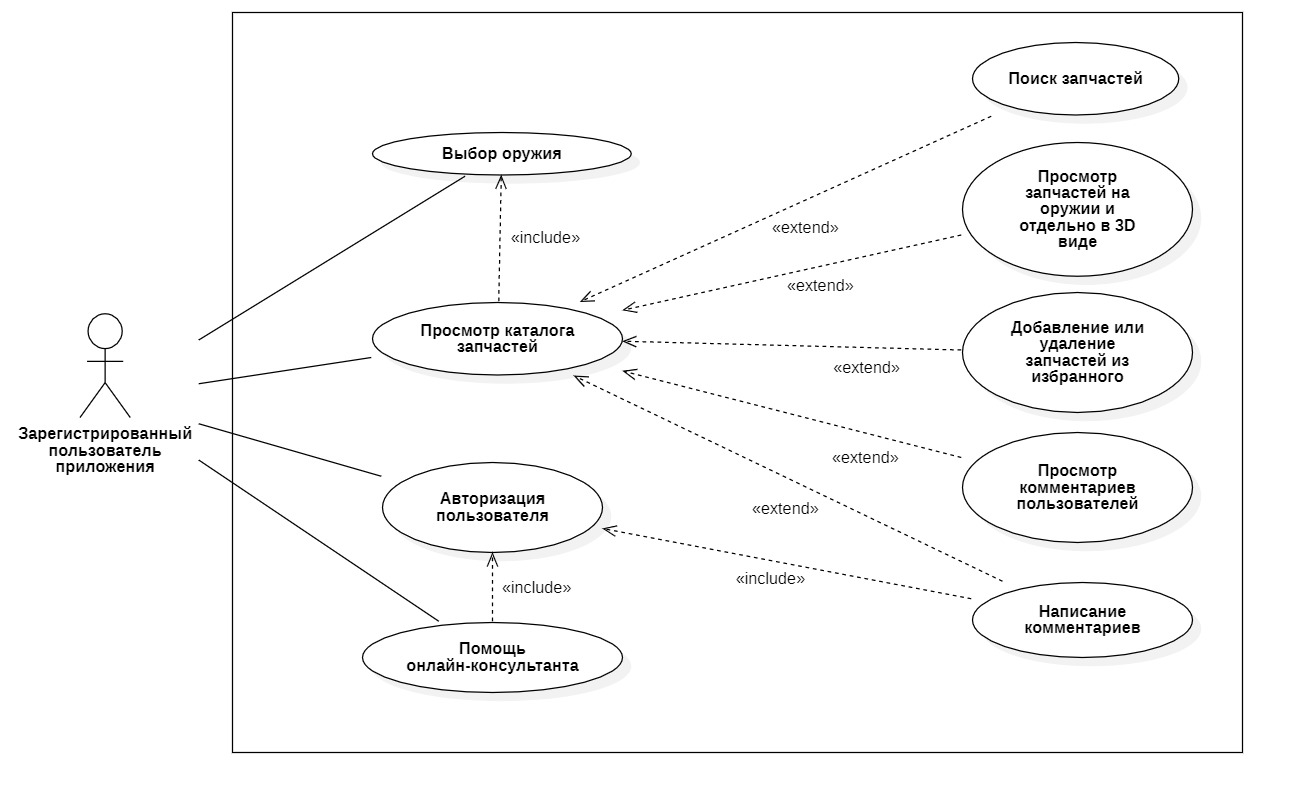
\includegraphics[width=1\linewidth]{reg}}
\caption{Диаграмма прецедентов для зарегистрированных пользователей}
\label{fig2}
\end{figure}

\begin{figure}[H]
\centerline{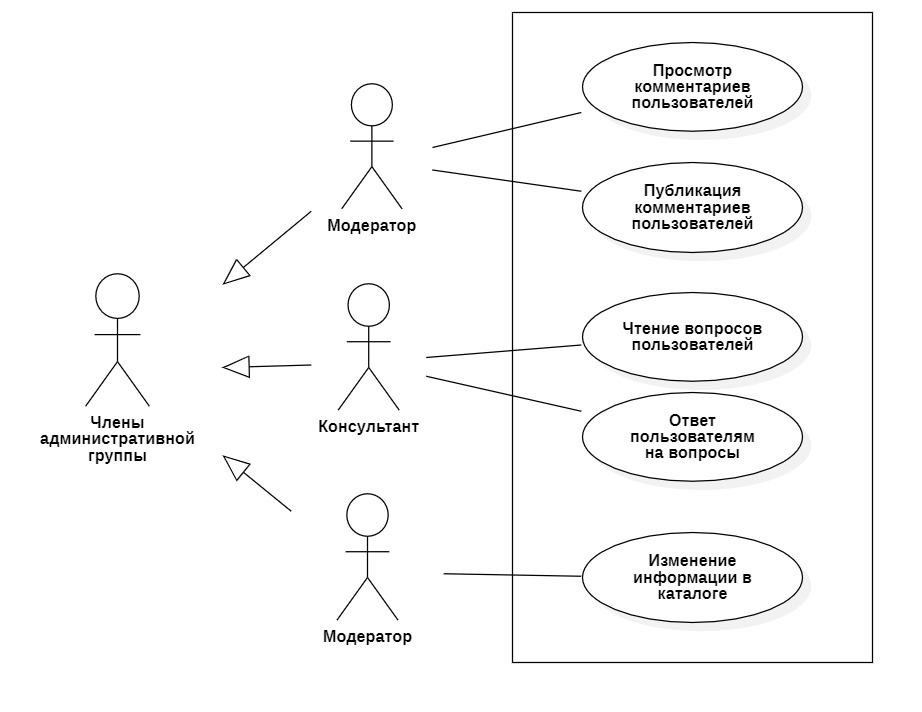
\includegraphics[width=0.7\linewidth]{adm}}
\caption{Диаграмма прецедентов для членов административной группы}
\label{fig3}
\end{figure}

\newpage
\section{Диаграммы активности для ключевых прецедентов}

В данном разделе представлены диаграммы активности для следующих прецедентов: авторизация пользователей (рисунок \ref{fig4}), использование каталога (рисунок \ref{fig5}), модерация комментариев (рисунок \ref{fig6}), помощь онлайн-консультанта (рисунок \ref{fig7}) и обновление менеджером информации в приложении (рисунок \ref{fig8}).

\begin{figure}[H]
\centerline{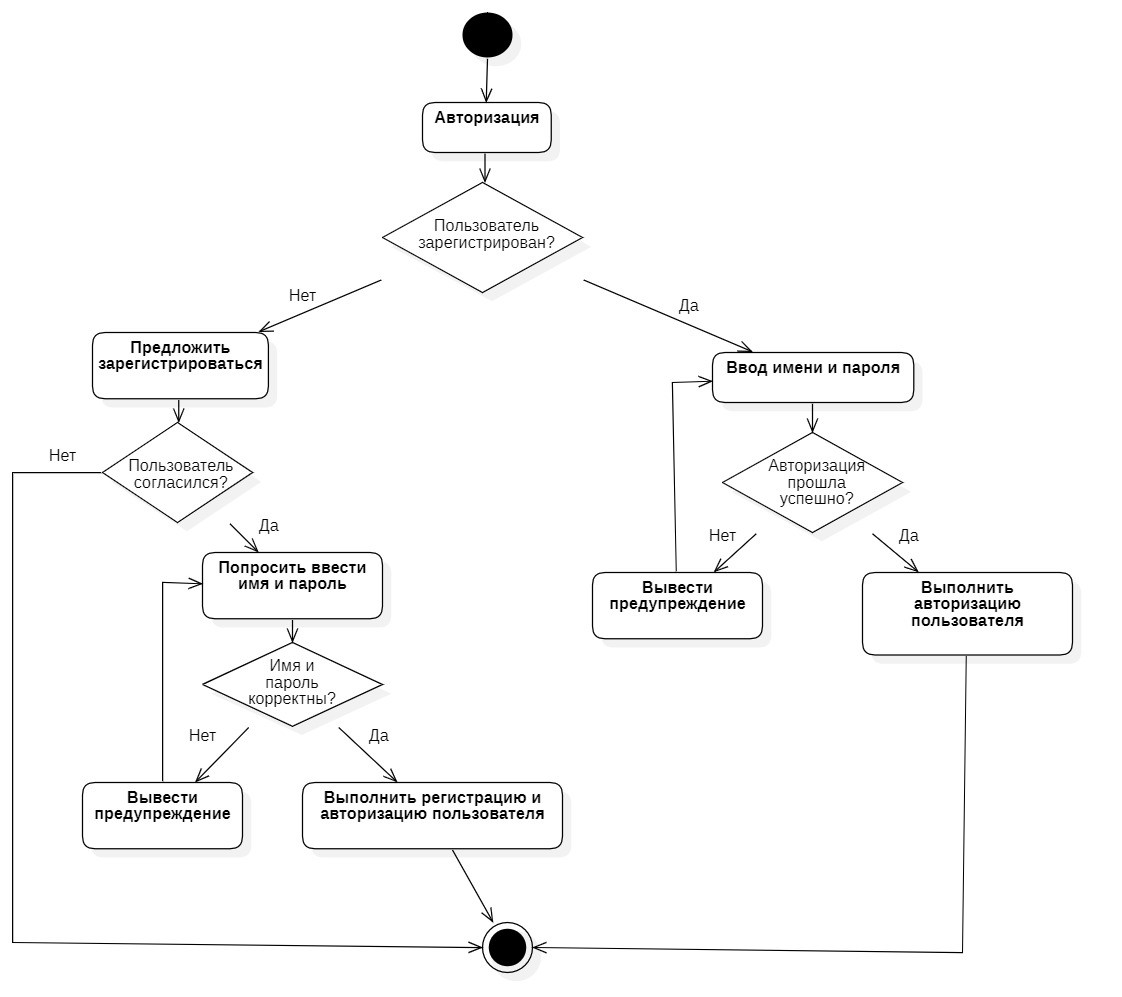
\includegraphics[width=1\linewidth]{act_avto}}
\caption{Диаграмма активности авторизации пользователей}
\label{fig4}
\end{figure}

\begin{figure}[H]
\centerline{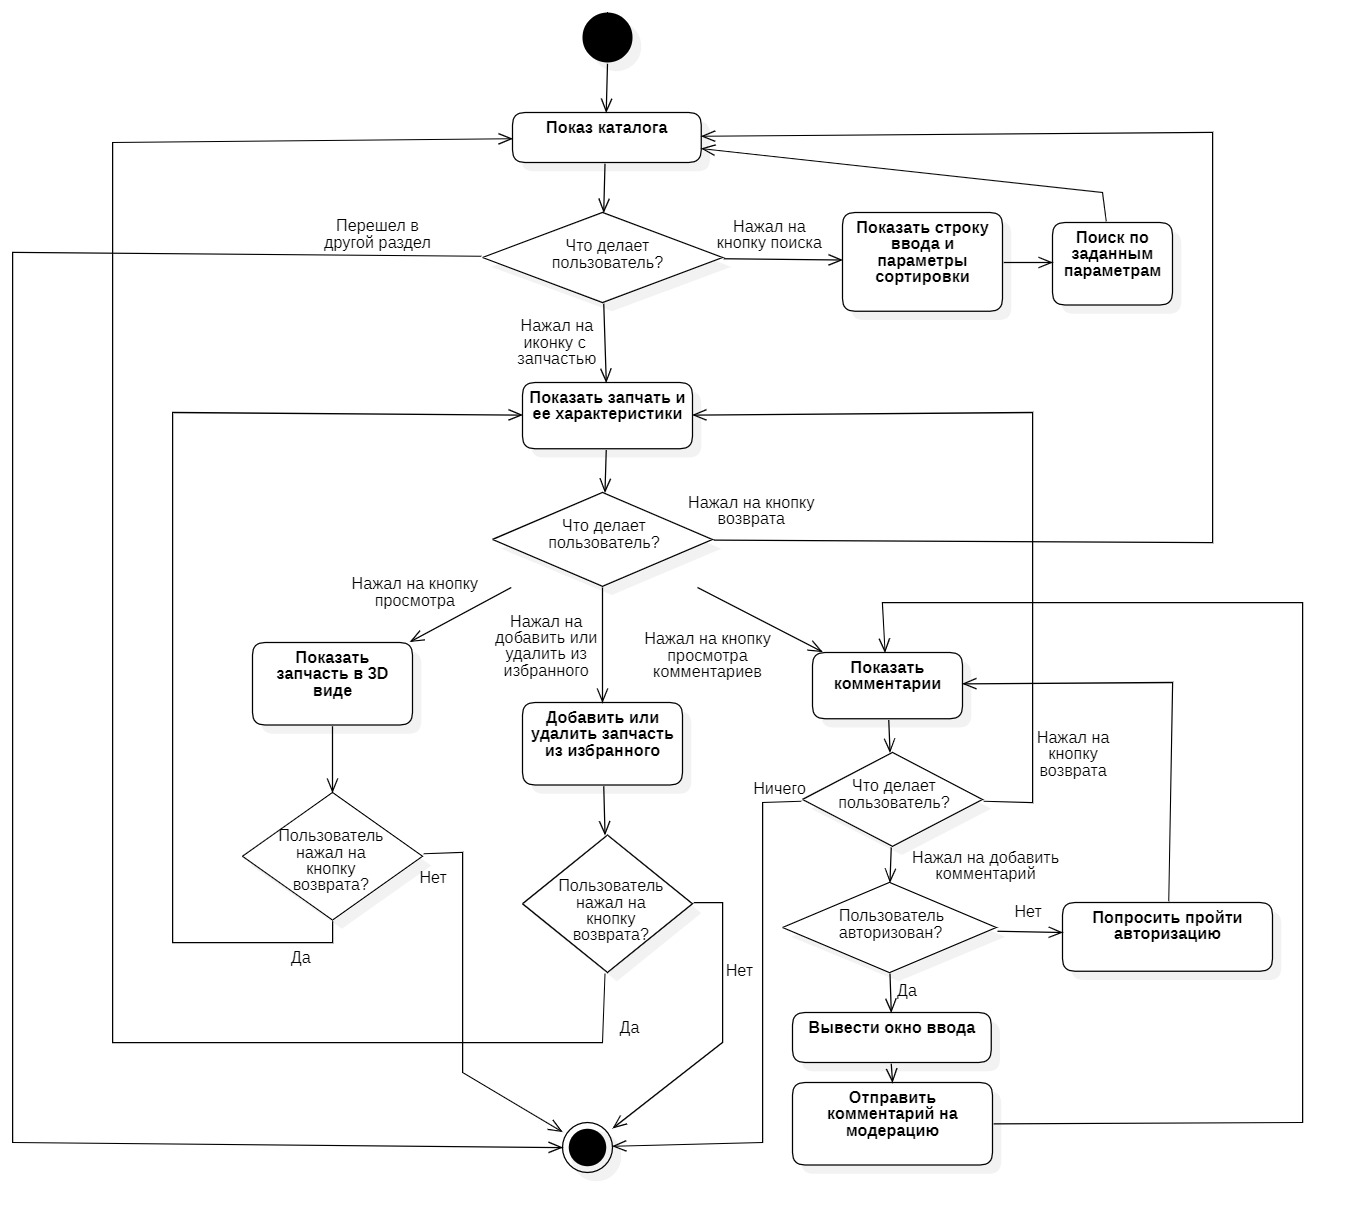
\includegraphics[width=1.05\linewidth]{act_pols}}
\caption{Диаграмма активности использования каталога пользователем}
\label{fig5}
\end{figure}

\begin{figure}[H]
\centerline{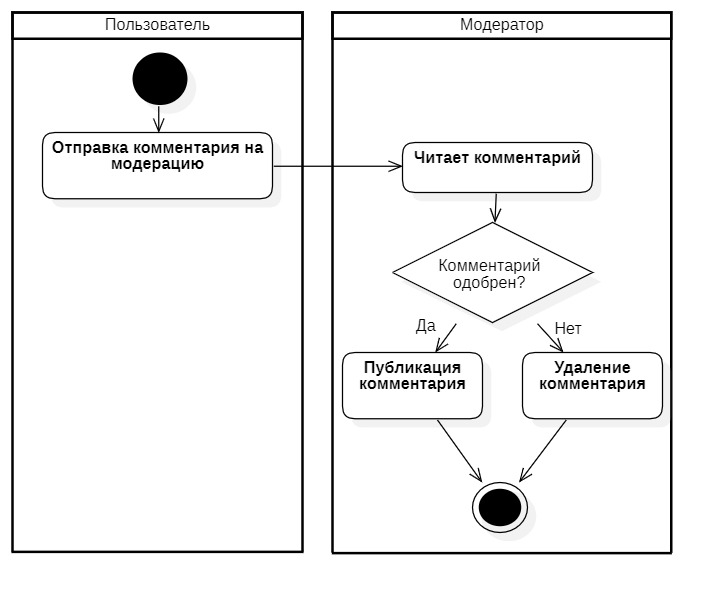
\includegraphics[width=0.7\linewidth]{act_kom}}
\caption{Диаграмма активности отправки комментария на модерацию}
\label{fig6}
\end{figure}

\begin{figure}[H]
\centerline{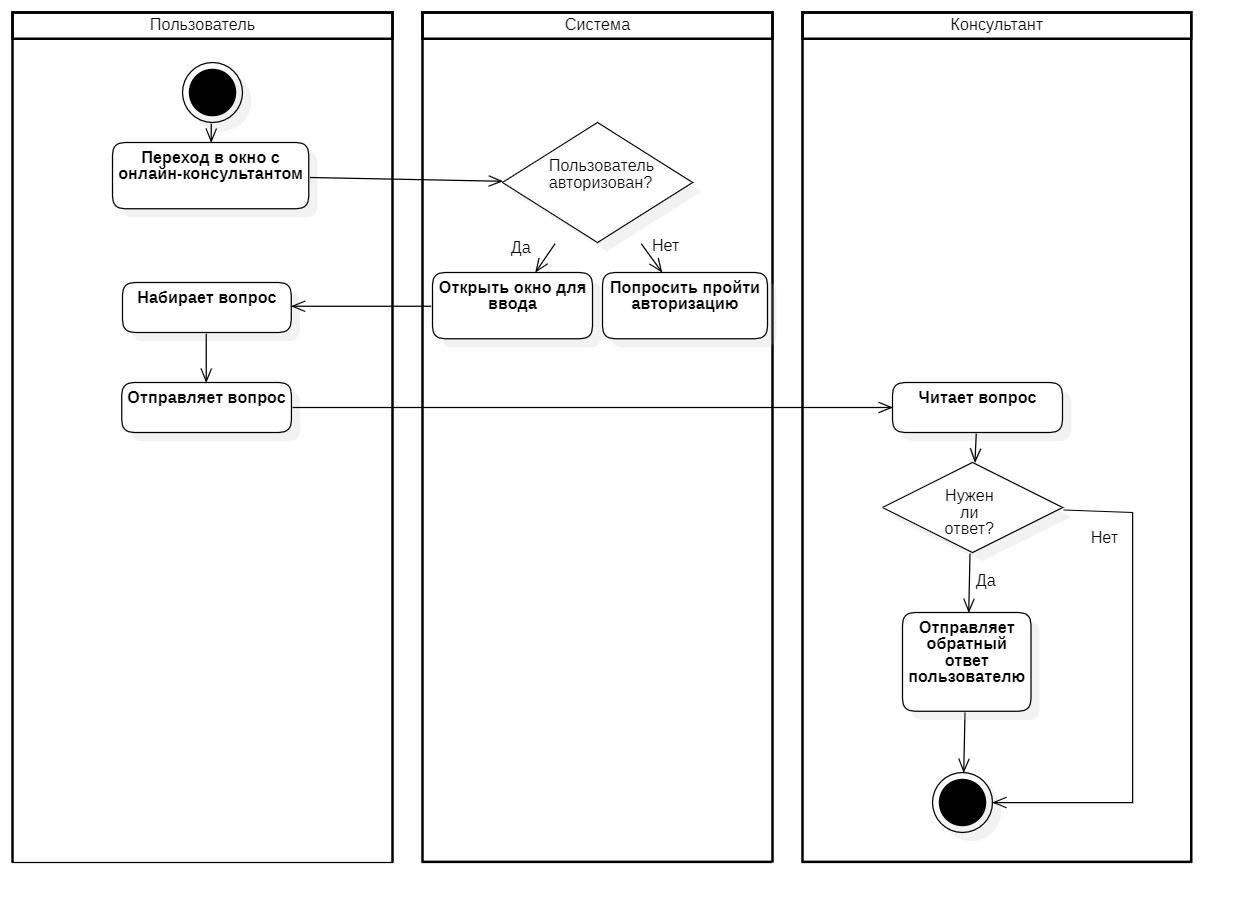
\includegraphics[width=1\linewidth]{act_kons}}
\caption{Диаграмма активности обращения к онлайн-консультанту}
\label{fig7}
\end{figure}

\begin{figure}[H]
\centerline{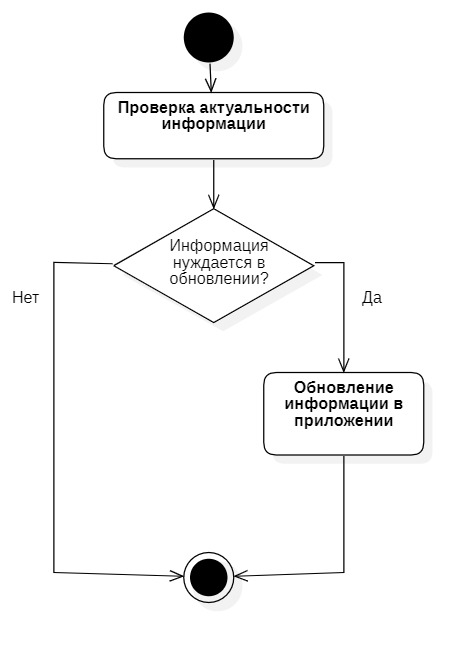
\includegraphics[width=0.5\linewidth]{act_men}}
\caption{Диаграмма активности обновления менеджером информации}
\label{fig8}
\end{figure}


\newpage
\section{Альтернативные потоки событий и исключения}

В данном разделе рассмотрены альтернативные потоки событий и исключения в виде таблиц для следующих вариантов использования: авторизация пользователя (таблица~\ref{table1}), поиск необходимой запчасти пользователем (таблица~\ref{table2}) и оставление комментария пользователем (таблица~\ref{table3}).

\begin{table}[H]

\begin{center}
\caption{Авторизация пользователя \label{table1}}
\begin{tabular}{|p{5.5cm}|p{10.7cm}|}
\hline
Вариант использования & Авторизация пользователя \\
\hline
Актеры
 & Пользователь
 \\
\hline
Цель
 & Авторизация в приложении для использования полного функционала 
 \\
\hline
Краткое описание
 & Приложение просит пользователя пройти авторизацию, далее, если пользователь зарегистрирован, он вводит имя и пароль, иначе пользователь может пройти регистрацию
 \\
\hline
Исключения
 & 
$\cdot$ Если пользователь зарегистрирован, то он может ввести неправильное имя или пароль

$\cdot$ Если пользователь незарегистрирован, то выбранное им имя уже может быть использовано
 \\
\hline
Альтернативный ход 

событий
& Пользователь может отказаться проходить авторизацию и сразу перейти к использованию приложения \\

\hline
\end{tabular}
\end{center}
\end{table}

\begin{table}[H]

\begin{center}
\caption{Поиск необходимой запчасти пользователем
 \label{table2}}
\begin{tabular}{|p{5.5cm}|p{10.7cm}|}
\hline
Вариант использования & Поиск необходимой запчасти
 \\
\hline
Актеры
 & Пользователь
 \\
\hline
Цель
 & Найти конкретную запчасть
 \\
\hline
Краткое описание
 & Пользователь переходит в раздел каталога и смотрит страницы, пока не найдет необходимую запчасть
 \\
\hline
Исключения
 &  В приложении нет информации о данной запчасти
 \\
\hline
Альтернативный ход 

событий
& Пользователь переходит в раздел каталога, нажимает на кнопку поиска, вводит имя запчасти и использует параметры сортировки, после чего находит необходимую запчасть
 \\

\hline
\end{tabular}
\end{center}
\end{table}
\begin{table}[H]
\begin{center}
\caption{Оставление комментария пользователем
 \label{table3}}
\begin{tabular}{|p{5.5cm}|p{10.7cm}|}
\hline
Вариант использования & Написание комментария
 \\
\hline
Актеры
 & Пользователь, модератор
 \\
\hline
Цель
 & Написать отзыв об использовании данного тюнинга
 \\
\hline
Краткое описание
 & Зарегистрированный пользователь переходит в раздел комментариев запчасти, о которой он хочет оставить отзыв, пишет комментарий и отправляет его на модерацию, после чего модератор одобряет комментарий и публикует его
 \\
\hline
Исключения
 &  У пользователя были проблемы со связью, поэтому комментарий не был отправлен
 \\
\hline
Альтернативный ход 

событий
&Комментарий был удален, так как модератор его не одобрил
 \\
\hline
\end{tabular}
\end{center}
\end{table}



\conclusions

Был составлен отчет, в котором были представлена диаграммы активности и вариантов использования мобильного приложения OptiTune на языке UML, а также были рассмотрены альтернативные потоки событий и исключения для основных прецедентов.



\newpage
\begin{thebibliography}{99}

\bibitem{bib1} Habr: официальный сайт. – URL: \url{https://habr.com/ru/post/566218/} (Дата обращения 28.10.2022).

\end{thebibliography}







\end{document}
